\subsection{Benchmarking for Employee Use Case}
(Maybe start text fancy with the questions which arise during the project: see the benchmarking google sheet for that)

As already mentioned this project was carried out as a prototyping project. Therefore we need to benchmark our results against the current best practice. Current state of the art for deploying contracts to the ethereum blockchain includes saving all the state variables of the contract on the blockchain and thus on all machines participating in the blockchain. As proposed we want to save those state variables off from the blockchain and thus save on gas which explains why gas cost are our most important measurement.

%- What did we benchmark?
%Explain which scenarios we did test (1 employee, multiple employee)
We especially benchmarked the employee use case as the employee use case is the more complex one of our both use cases. As a preparation for benchmarking we first needed two different smart contracts. One smart contract that works completely on-chain without using any external database, hashing functions or merkle trees and another smart contract that uses all introduced methods that are needed in order to off-chain our data to an external database. The two variants behave completely similar except for the saving of the state variables. Both variants are completely functional and could be used as they are if someone would like to deploy the employee use case. These fact were very important to us because only like that we could make sure that our benchmarks lead to meaningful results. Within the employee use case we measured different scenarios which will be described in the corresponding sections, mainly a time measure as well as a simple and another complex measure for the gas cost have been made.

%Explain under which aspects we did benchmark (gas, time)
%Mention again why gas is of utmost importance to us (because it translates to money and time)
%Explain the thing with benchmarking only the overhead due to automining of ganache
We mainly benchmarked the two measurements gas cost and time. Gas cost was the initial motivation for off-chaining as we assumed to save on gas cost when we off-chain the state variables. Gas cost translates to real currency as a participant of the blockchain either needs to buy Ether or help to mine blocks in order to receive Ether which is needed to pay the resulting gas cost of a transaction. The time was measured as we wanted to gain insights into how much overhead our application adds to a normal blockchain application. This was possible as our technology stack includes ganache which is capable of automatically mining new transactions into new blocks instantly so that we are able to measure only the overhead that our application introduces.

%- Nice transition into showing our first graphics.
\subsubsection{Time measurement}
First we will measure the introduced computation time of our application for executing different functions of the smart contract. The result can be seen in Figure \ref{fig:05_time}.

\begin{figure}[t]%evtl:[t] [!htbp]
\centering
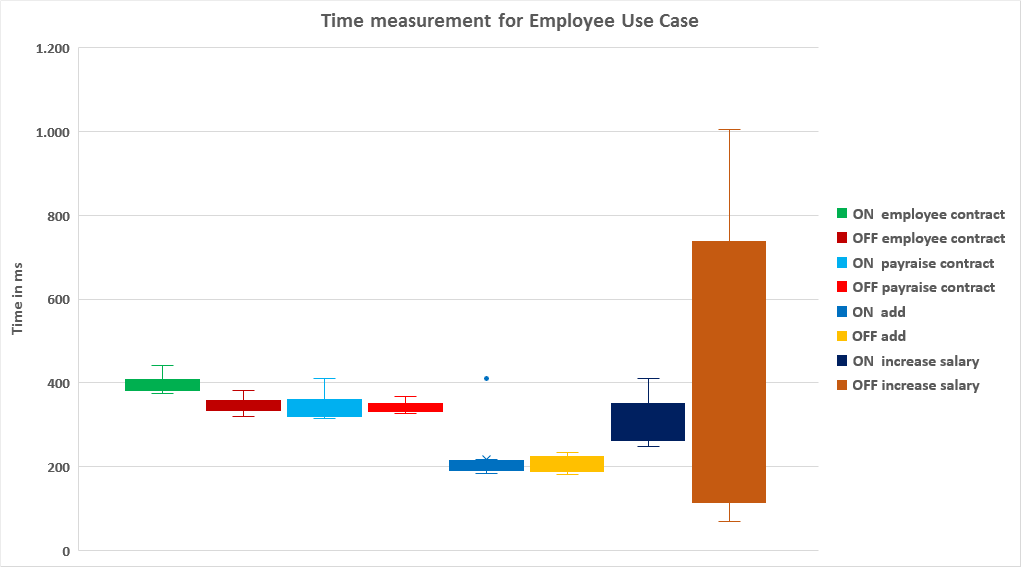
\includegraphics[width=1.0\textwidth]{images/05_evaluation/05_time.png}
\caption{\label{fig:05_time}Time measurement for Employee Use Case.}
\end{figure}

%Thats a box plot chart
As we measured the computation time multiple times we decided to unite the results into a box plot chart. Thus we can see how the system behaves most of the times and single outliers can easily be identified. Throughout our measurement we always compare the on-chained approach against the off-chained approach. Every single function got called multiple times and the results have been summed up into the corresponding box plot.

For the \textit{employee contract} creation we can see the that the time differs by circa 50ms when comparing the on-chained approach to the off-chained approach. The on-chained approach needs about 400ms of computation time in the application while the off-chained approach needs 350ms. Both timings are negligible for us as the average block time of the ethereum blockchain is currently about 14 seconds [TODO: Need citation: https://etherscan.io/chart/blocktime]. Thus our application has more than enough time to compute a new transaction comparing nearly half a second against 14 seconds.

The \textit{payraise contract} creation needs about the same time for the on-chained as for the off-chained approach. Both need about 350ms of computation time and are negligible for the same reason as for the \textit{employee contract} creation. The same holds true for the \textit{add} functionality which takes even less time and thus the timing is negligible here as well.

More interesting are the timing needs of the \textit{increase salary} functionality. We can easily see that the off-chained variant has a much higher variance than the on-chained variant and we have peeks in the computation time of up to one second. Hereby it is very important to mention that the time needed for the off-chained variant increases with the size of the employee dataset. This happens because for every added employee the \textit{increase salary} function needs to generate another transaction. As every transaction needs to be mined first the increased timing needs of our application are also negligible as what we see in our chart is the cumulated computation time for all transactions that happened during this function call. All of these transactions need to be mined within blocks of the ethereum blockchain which takes a lot longer, namely about 14 seconds currently, than the computation of our application. Plus, it could possibly happen that the single transactions will be divided on multiple blocks. Therefore the introduced timing needs of our application are also negligible for this function and additionally all measurements of the \textit{increase salary} function were less than a second which is quite fast.% maybe explain that the introduced overhead is somehow "virtual?"

%Everything under 1 second -> not relevant, no further measurements
%Erwähnen dass es super ist, dass die middlewar keine extra zeiten introduced und genauso fix ist wie das normale.
As every function call in the off-chained approach does not introduce a real overhead compared to the on-chained approach and our application always performed under one second we concluded that we do not need to deeper analyze what introduces the most computation time or how to optimize for time in our application as this would not include a great benefit for our use case. Therefore no further measurements concerning the computation time have been made. We can conclude that the off-chained approach did not introduce any additional computation time and is as good as the on-chained approach timewise.

\subsubsection{Gas cost measurement}
Measuring the gas needed for executing the functionalities of our smart contract is of utmost importance to us. The initial motivation for our prototype was to gain experience on whether it is possible to save on gas cost when off-chaining state variables from smart contracts. As we receive the used gas for each transaction within the JSON-response when we call the smart contract functions through our API endpoint we were able to extract different insights into the use of gas when on- or off-chaining.

%And smth more in Figure \ref{fig:05_gas_cost_single}.
In Figure \ref{fig:05_gas_cost_single} we visualized the used gas for calling single functions of our smart contract for the employee use case. Similarly to our time measurement we again measured the main functionalities of our smart contract and compared the on-chained variant with the off-chained variant.

\begin{figure}[t]
\centering
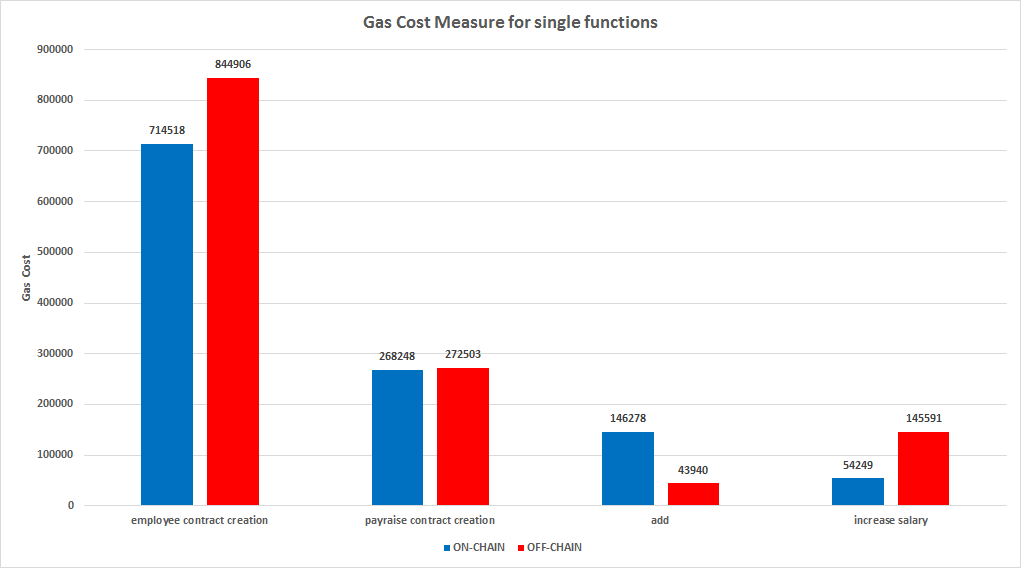
\includegraphics[width=1.0\textwidth]{images/05_evaluation/05_gas_cost_single.png}
\caption{\label{fig:05_gas_cost_single}This is one employee.}
\end{figure}

- employee creation more costy because overhead of functions for merkle tree (ellaborate what exactly here)

% 844906 - 714518 = 130388 gas,    130388 / 714518 = 18,25%
For the employee contract creation we can see that the off-chained variant needs about 130 thousand less gas than the on-chained variant. Say why we save and then in the end say that its constant and how much percentage-wise this translates to

- payraise not changed (on-chained for both, thats why it is the same)

- on add we save xy gas because thats where off-chaining is stronk

- increase salary we loose because [.....] only one field, multiple transactions, ellaborate on possible alternatives like functions that would change multiple strings etc etc

And yet smth more in Figure \ref{fig:05_gas_cost_ten}.

\begin{figure}[htbp]
\centering
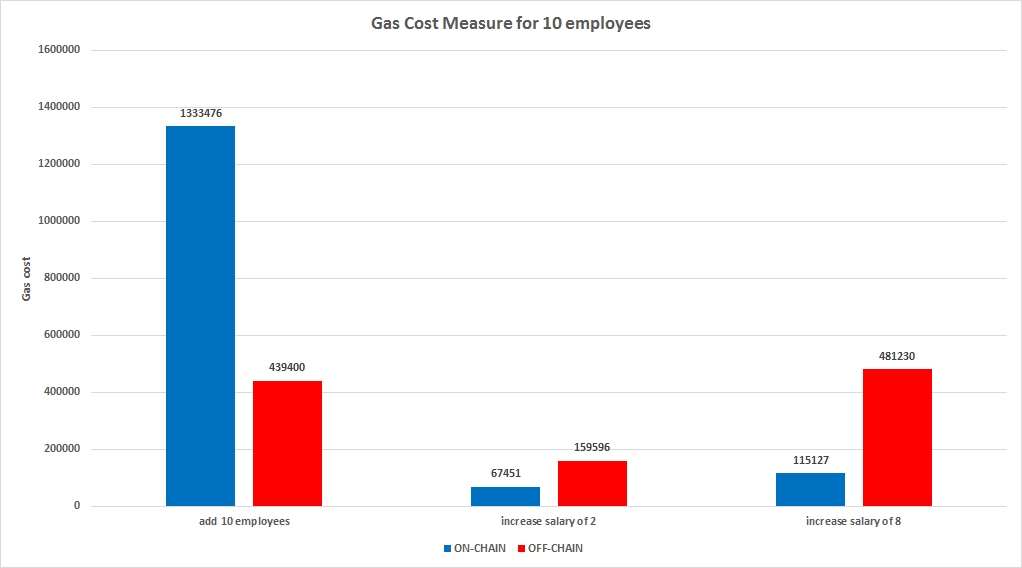
\includegraphics[width=1.0\textwidth]{images/05_evaluation/05_gas_cost_ten.png}
\caption{\label{fig:05_gas_cost_ten}This is ten employees.}
\end{figure}



- Insert graphics / statistics

Explain what is visible

Explain what that does mean

- Ellaborate on conclusions and findings from this evaluation

What do all the statistics say? what do they mean to us?

When does Off-Chaining make sense?

Do we really save gas?

- Later on say how our measurements can be compared to the financials use case (cut out the increase-salary basically)

- Know your use case!

- Give pay-raise as example for when off-chaining makes no sense (we kept it on-chain)

-> Conclude on that
